% !TeX program = pdflatex
\documentclass[tikz,border=8pt]{standalone}
\usepackage{tikz}\usetikzlibrary{angles,quotes,calc}
\definecolor{FigureBlue}{HTML}{2563EB}\definecolor{FigureOrange}{HTML}{EA580C}
\begin{document}
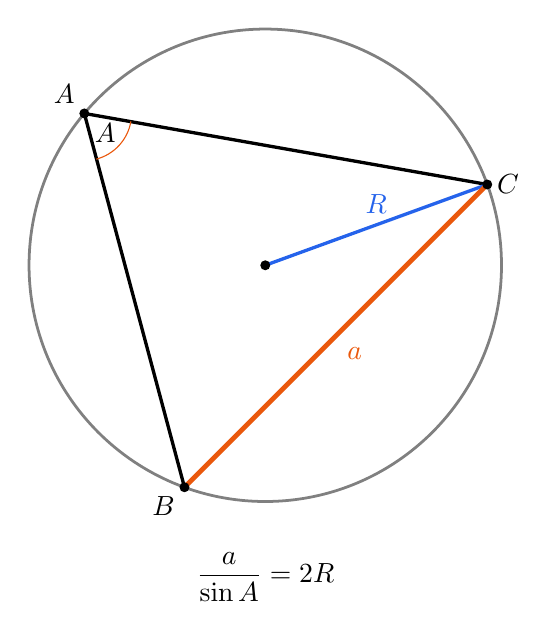
\begin{tikzpicture}[line cap=round,line join=round]
  \coordinate (O) at (0,0); \coordinate (A) at (140:3); \coordinate (B) at (250:3); \coordinate (C) at (20:3);
  \draw[gray,line width=1pt] (O) circle (3); \draw[line width=1.2pt] (A)--(B)--(C)--cycle;
  \draw[FigureBlue,line width=1.2pt] (O)--(C) node[midway,above] {$R$};
  \draw[FigureOrange,line width=1.7pt] (B)--(C) node[midway,below right] {$a$};
  \pic[draw=FigureOrange,angle radius=6mm,"$A$"] {angle=B--A--C};
  \fill (O) circle (1.8pt); \foreach \P in {A,B,C}{\fill (\P) circle (1.8pt);}
  \node[above left] at (A) {$A$}; \node[below left] at (B) {$B$}; \node[right] at (C) {$C$};
  \node[below=7mm] at (O |- B) {$\displaystyle\frac{a}{\sin A}=2R$};
\end{tikzpicture}
\end{document}
